\section{Sec.~I: Introduction and Motivations}

\subsection{What problem is this paper actually solving?}

Before any equation, it helps to say in plain words what question this whole 119-page paper is an answer to,
because the paper itself takes a few pages of fairly compressed language to say it, and it's easy to lose the
forest for the trees once the algebra starts.

Here is the question. Ordinary physics — both classical and quantum — treats spacetime as a fixed stage:
space and time are given in advance, with a definite geometry (flat, or curved according to some metric),
and physics happens \emph{on} that stage. General relativity already complicates this a little, because the
geometry itself is dynamical (matter tells spacetime how to curve, spacetime tells matter how to move), but
even there, at any given moment you can ask ``what is the metric right here'' and get a sharp, well-defined
answer. Quantum gravity is the attempt to quantize this whole picture — and the moment you do, the metric
itself becomes an operator, subject to quantum fluctuations, and the question ``what is the geometry right
here'' stops having a sharp answer in the same way that ``where exactly is the electron'' stops having a
sharp answer once you quantize a particle's position. Geometric concepts like ``this point is to the future
of that point,'' or ``this region is causally connected to that region,'' or ``this is a local, self-contained
patch of space'' — all of these are only sharply defined in the classical limit, which physicists write as
$G_N\to0$ ($G_N$ is Newton's gravitational constant; turning it off turns off quantum-gravitational effects
and leaves you with an ordinary, fixed classical geometry).

So here is the actual research question the paper poses: suppose you are handed a complete quantum theory of
gravity at some finite, nonzero $G_N$ — no classical geometry assumed, no metric given in advance, nothing
geometric built in from the start. As you dial $G_N\to0$, familiar geometric structures (a well-defined
notion of ``here,'' of causal order, of a local region) are supposed to emerge. \textbf{What, physically and
mathematically, is doing the emerging?} What is it about the underlying quantum theory that produces
spacetime geometry as $G_N\to0$, and what role, if any, does quantum entanglement play?

This is not an idle question. The clearest place it can be asked precisely is the AdS/CFT correspondence,
where a theory of quantum gravity living in a $(d{+}1)$-dimensional \emph{anti-de Sitter} spacetime (AdS,
a spacetime with constant negative curvature, chosen because it has a well-defined boundary at infinity) is
conjectured to be completely equivalent to an ordinary, non-gravitational quantum field theory — a
\emph{conformal field theory} (CFT) — living on that $d$-dimensional boundary. On the CFT side, there is a
parameter $N$ that counts the number of independent field degrees of freedom (originally, for the gauge
theories where this was first understood, $N$ was literally the number of colors of an $SU(N)$ gauge group).
The AdS/CFT dictionary says $G_N$ on the gravity side maps to a positive power of $1/N$ on the CFT side, so
$G_N\to0$ (classical, geometric gravity) is exactly the same limit as $N\to\infty$ on the boundary. The
question above becomes concrete and answerable: \emph{how does bulk spacetime — its geometry, its causal
structure, its locality — emerge from an ordinary quantum field theory living on a lower-dimensional boundary,
as that boundary theory's number of degrees of freedom is sent to infinity?}

The Ryu--Takayanagi proposal (2006) was the first strong hint at the answer: it conjectures a formula tying
the entanglement entropy of a boundary region to the area of a certain minimal surface in the bulk — literally
an equation relating an entanglement measure to a geometric quantity. If entanglement entropy and bulk area
are related this tightly, entanglement itself must be doing real structural work in building the bulk
geometry, not just decorating it. That is the motivating intuition. The rest of the paper is the attempt to
make this intuition completely precise, and the tool that does it turns out to be a piece of 1930s
mathematics — von Neumann algebras — that was originally developed for a completely different reason (putting
ordinary quantum mechanics on a rigorous footing), and has only recently been recognized as exactly the right
language for this question.

\begin{table}[t]
\centering
\footnotesize
\begin{tabularx}{\textwidth}{@{}l p{4.8cm} X@{}}
\toprule
\textbf{Symbol / Structure} & \textbf{Mathematical Definition} & \textbf{Physical Interpretation / Role} \\
\midrule
$\HH$ & Global Hilbert space of states & Total state space of the universe / system \\
$B(\HH)$ & Bounded linear operators on $\HH$ & All bounded operations and observables \\
$\M \subset B(\HH)$ & von Neumann algebra ($\M = \M''$) & Observables accessible to a local subregion / observer \\
$\M'$ & Commutant: $\{B : [B,A]=0\ \forall A \in \M\}$ & Observables of the causal complement / independent subsystem \\
$\mathcal{Z}(\M) = \M \cap \M'$ & Center of the algebra & Classical superselection sectors (trivial $\mathbb{C}\id$ for factors) \\
$\omega: \M \to \mathbb{C}$ & State (positive linear functional, $\omega(\id)=1$) & Expectation value functional $\omega(A) = \langle A \rangle$ \\
$(\pi_\omega, \HH_\omega, \ket{\Omega_\omega})$ & GNS representation & Hilbert space manufactured directly from state $\omega$ \\
$\ket\Psi \in \HH$ & Cyclic \& separating vector & Entangled vacuum / state with no local annihilators \\
$S_\Psi$ & Tomita antilinear operator: $S_\Psi A\ket\Psi = A^\dagger\ket\Psi$ & State-dependent modular involution \\
$J_\Psi$ & Modular conjugation ($J_\Psi \M J_\Psi = \M'$) & Antilinear reflection mapping algebra to its commutant (e.g. CPT) \\
$\Delta_\Psi = S_\Psi^\dagger S_\Psi$ & Modular operator ($\Delta_\Psi > 0$, self-adjoint) & Relative entanglement density / asymmetry operator \\
$h_\Psi \equiv -\log\Delta_\Psi$ & Modular Hamiltonian & Generator of intrinsic subsystem time flow (e.g. Rindler boost) \\
$\sigma_t^\Psi(A) = \Delta_\Psi^{it} A \Delta_\Psi^{-it}$ & Modular flow ($1$-parameter automorphism) & Thermal time evolution satisfying the KMS condition \\
$\widehat\M = \M \rtimes_\sigma \mathbb{R}$ & Crossed product algebra with clock $L^2(\mathbb{R})$ & Gravitationally dressed algebra including observer energy/clock \\
$\tau$ & Semifinite trace on $\widehat\M$ ($\tau(AB)=\tau(BA)$) & Renormalized trace yielding well-defined density matrices \\
$S_{\rm gen}$ & Generalized entropy: $\frac{\langle \hat A\rangle}{4G_N} + S_{\rm bulk}$ & Finite gravitational entropy in semiclassical gravity \\
$\mathcal{A}_{\rm CFT}$ & Boundary single-trace algebra ($N\to\infty$) & Generalized free fields on the holographic boundary \\
$\mathcal{A}_{\rm bulk}(b_A)$ & Bulk algebra in entanglement wedge $b_A$ & Local semiclassical bulk quantum fields dual to boundary region \\
\bottomrule
\end{tabularx}
\caption{Summary of core notation, algebraic structures, and physical interpretations used throughout this companion.}
\label{tab:notation_summary}
\end{table}

\begin{figure}[htbp]
\centering
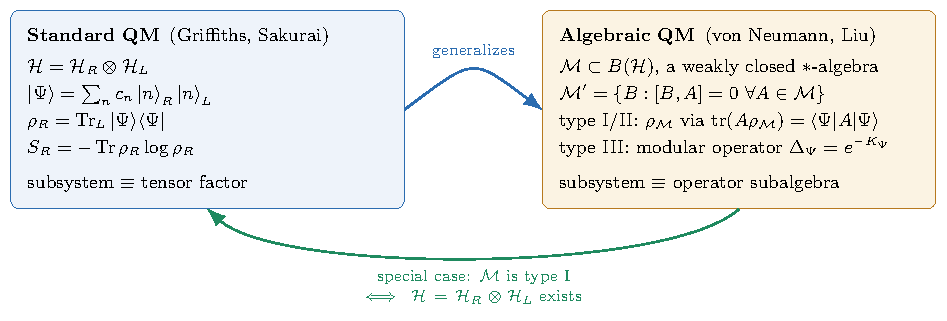
\includegraphics[width=0.92\textwidth]{figs/fig_roadmap.pdf}
\caption{The foundational paradigm shift: Standard Hilbert space quantum mechanics (left, where subsystems are defined by tensor factors $\HH = \HH_R \otimes \HH_L$) generalizes to Algebraic Quantum Mechanics (right, where subsystems are defined by operator subalgebras $\M \subset B(\HH)$). Type I algebras represent the familiar special case where a tensor product factorization exists.}
\label{fig:roadmap}
\end{figure}

\subsection{The Conceptual Bridge: From Wavefunctions to Density Matrices to Algebraic States}

To understand why the algebraic framework of this paper is so natural, it is essential to trace how our concept of a ``quantum state'' evolves as we move from simple undergraduate quantum mechanics to open systems, quantum field theory, and quantum gravity.

\begin{enumerate}[leftmargin=*]
\item \textbf{Level 0: The Pure Wavefunction $\psi(x) = \braket{x|\Psi}$.}
In textbook quantum mechanics, the fundamental entity is a state vector $\ket\Psi \in \HH$ evolving according to the Schr\"odinger equation. Probabilities are given by the Born rule $P(x) = |\psi(x)|^2$. This description assumes a \emph{closed, isolated universe} where an experimenter has unrestricted access to measure arbitrary operators across the entire system.

\item \textbf{Level 1: The Density Matrix $\rho(x, x')$ and Phase Space ($x_c, x_q$).}
When a system interacts with an unobserved environment or thermal bath, pure states give way to density operators $\rho = \sum_k p_k \ket{\psi_k}\bra{\psi_k}$. In the continuous position basis $\rho(x, x') = \braket{x|\rho|x'}$, it is physically illuminating to transform to Keldysh variables:
\[
x_c \equiv \frac{x + x'}{2} \quad \text{(classical midpoint coordinate)}, \qquad x_q \equiv x - x' \quad \text{(quantum coherence coordinate)}.
\]
The diagonal slice $x_q = 0$ encodes classical probabilities $P(x_c) = \rho(x_c, x_c)$, while non-zero $x_q$ tracks off-diagonal quantum interference. Fourier transforming along the quantum coordinate gives the \textbf{Wigner quasi-probability distribution}:
\[
W(x_c, p_q) = \int_{-\infty}^\infty \dd x_q\, e^{-i p_q x_q}\, \rho\!\left(x_c + \tfrac{x_q}{2},\, x_c - \tfrac{x_q}{2}\right) .
\]
While this bridges classical stochastic physics and quantum mechanics, it still fundamentally presumes that the global Hilbert space factorizes as $\HH = \HH_{\rm system} \otimes \HH_{\rm environment}$.

\item \textbf{Level 2: The Physical Limitation of Observers.}
In realistic experiments, no observer has access to the full density matrix on all of $\HH$. An observer is equipped with a restricted apparatus or confined to a spatial subregion $R$. If an observer can only measure a restricted set of observables $\M$, attempting to describe their subsystem via global pure kets produces severe mathematical pathologies (for instance, the standard relative entropy $D(\rho\|\sigma) = \Tr(\rho\log\rho - \rho\log\sigma)$ formally blows up to $+\infty$ whenever $\sigma$ is pure, because it assumes the observer is free to measure arbitrary non-commuting projection operators across the universe).

\item \textbf{Level 3: The Algebraic State $\omega: \M \to \mathbb{C}$.}
In algebraic quantum mechanics (von Neumann, Haag, and Liu), we discard the assumption that a fixed global Hilbert space is fundamental. The primary physical object is the \textbf{algebra of accessible observables $\M$}. A \textbf{state} $\omega$ is simply a positive linear functional assigning expectation values to operators:
\[
\omega(A) = \langle A \rangle_\omega, \qquad \omega(\id) = 1, \quad \omega(A^\dagger A) \ge 0 \quad \forall A \in \M.
\]
The Hilbert space $\HH_\omega$ and state vector $\ket{\Omega_\omega}$ are not postulated in advance; they are \textbf{dynamically manufactured} from the algebraic state $\omega$ via the Gelfand--Naimark--Segal (GNS) construction:
\[
\omega(A) = \braket{\Omega_\omega | \pi_\omega(A) | \Omega_\omega} .
\]
\end{enumerate}

\begin{keyresult}
\textbf{The Conceptual Takeaway:} The wavefunction $\psi(x)$ is not a universal container of physical reality; it is merely one specific GNS representation of an algebraic state $\omega$ on a Type I algebra. When moving to the thermodynamic limit ($N\to\infty$), local subregions in QFT, or semiclassical black holes, the Hilbert space tensor factorization dissolves, but the algebraic state $\omega$ remains exact, rigorous, and well-defined.
\end{keyresult}

\subsection{Why the ordinary quantum-mechanical definition of ``subsystem'' isn't good enough}

To see why a new mathematical tool is needed at all, you have to see precisely where the old one breaks. The
old tool is the one from every quantum mechanics course: given a system built out of two pieces, $R$ and $L$
(read them as ``right'' and ``left,'' or ``region'' and its complement — any bipartition), the Hilbert space of
the whole system factors as a tensor product,
\[
\HH = \HH_R\otimes\HH_L .
\]
Concretely, if $\HH_R$ has orthonormal basis $\{\ket i_R\}$ and $\HH_L$ has orthonormal basis
$\{\ket a_L\}$, then $\HH_R\otimes\HH_L$ is spanned by all the pairs $\ket i_R\ket a_L$, and a general state of
the joint system is a sum $\ket\Psi = \sum_{ia} c_{ia}\ket i_R\ket a_L$ for some array of complex numbers
$c_{ia}$ (Liu's eq.~1.1, written with a continuous or more general index set — the idea is identical). This
state is called \textbf{entangled} exactly when the array $c_{ia}$ cannot be written as a simple product
$c_{ia}=\psi_i\chi_a$ for two smaller arrays $\psi_i,\chi_a$ — i.e., when it doesn't factor into ``something
about $R$'' times ``something about $L$.''

Everything about entanglement that you already know — the reduced density matrix
$\rho_R\equiv\Tr_L\ket\Psi\!\bra\Psi$ (tracing out, i.e., summing over, the $L$ degrees of freedom), the
entanglement entropy $S_R=-\Tr_R(\rho_R\log\rho_R)$, the R\'enyi entropies, the relative entropy — every one
of these formulas (Liu's eqs.~2.2--2.4) is built directly on top of the tensor factorization
$\HH=\HH_R\otimes\HH_L$. If that factorization doesn't exist, none of these formulas can even be written down,
because there is no $\HH_L$ to trace over and no well-defined ``$R$-part'' of the state to extract. The whole
apparatus of entanglement entropy that you learned collapses at the first step, not because it gives a wrong
answer, but because it has no answer to give.

The paper's central claim — the one that everything else builds on — is that this factorization genuinely
fails to exist, not as some exotic mathematical pathology, but in exactly the situations that matter most:
gauge theories, many-body systems in a thermodynamic (infinite-volume or infinite-$N$) limit, quantum field
theories cut into two regions by a surface, and — the case this paper cares about most — the large-$N$ limit
of a holographic boundary theory. Section~II.A of the paper (and this companion's next section) works through
three concrete examples of exactly how and why it fails. It is worth working through the second of these three
examples slowly and completely here, in Sec.~I, because it is the single example every later section in the
paper keeps coming back to.

\subsection{The example that carries the whole paper: infinitely many entangled qubit pairs}

Take a single pair of qubits, one belonging to $R$ and one to $L$, prepared in the state
\[
\ket{\phi_\theta} = \cos\theta\,\ket0_R\ket0_L + \sin\theta\,\ket1_R\ket1_L , \qquad \theta\in(0,\pi/4] .
\]
This is completely standard material: it's a partially entangled pair (maximally entangled exactly at
$\theta=\pi/4$, where the coefficients become equal, $\tfrac1{\sqrt2}$ each — this is a Bell pair). You could
build this in a lab tomorrow with two photons or two trapped ions. Nothing about a single pair is
mysterious.

To see the reduced density matrix explicitly, write out the full $4\times4$ density operator for the pure pair:
\[
\ket{\phi_\theta}\bra{\phi_\theta} = \cos^2\theta\ket{00}\bra{00} + \cos\theta\sin\theta\ket{00}\bra{11} + \sin\theta\cos\theta\ket{11}\bra{00} + \sin^2\theta\ket{11}\bra{11} .
\]
Now take the partial trace over subsystem $L$ by summing over the orthonormal basis $\{\ket0_L, \ket1_L\}$:
\begin{align*}
\rho_R &\equiv \Tr_L\ket{\phi_\theta}\bra{\phi_\theta} = {}_L\braket{0|\phi_\theta}\bra{\phi_\theta}0\rangle_L + {}_L\braket{1|\phi_\theta}\bra{\phi_\theta}1\rangle_L \\
&= \cos^2\theta\,\ket0_R\bra0_R + \sin^2\theta\,\ket1_R\bra1_R = \begin{pmatrix} \cos^2\theta & 0 \\ 0 & \sin^2\theta \end{pmatrix} .
\end{align*}
Because $\rho_R$ is already diagonal, its operator logarithm is obtained by taking the logarithm of each eigenvalue along the diagonal:
\[
\log\rho_R = \begin{pmatrix} \log(\cos^2\theta) & 0 \\ 0 & \log(\sin^2\theta) \end{pmatrix} .
\]
The single-pair von Neumann entanglement entropy follows immediately by evaluating the trace:
\begin{align*}
s_1(\theta) &= -\Tr_R(\rho_R\log\rho_R) = -\left[ \cos^2\theta\log(\cos^2\theta) + \sin^2\theta\log(\sin^2\theta) \right] .
\end{align*}
Evaluating at key points:
\begin{itemize}
\item For the maximally entangled Bell pair at $\theta=\pi/4$, $\cos^2(\pi/4)=\sin^2(\pi/4)=1/2$, yielding
\[
s_1(\pi/4) = -\left[ \tfrac12\log(\tfrac12) + \tfrac12\log(\tfrac12) \right] = \log 2 \approx 0.693147\text{ nats} \quad (= 1\text{ bit}).
\]
\item In the weakly entangled limit $\theta \to 0$, with $\sin^2\theta \approx \theta^2$ and $\cos^2\theta \approx 1 - \theta^2$:
\[
s_1(\theta) \approx -(1-\theta^2)\log(1-\theta^2) - \theta^2\log(\theta^2) \approx \theta^2(1 - 2\log\theta) \to 0 .
\]
\end{itemize}

Now take $N$ independent copies of this pair — $N$ separate two-qubit systems, each prepared the same way —
and glue them together into one big state:
\[
\ket{\Phi_\theta} = \ket{\phi_\theta}_1\otimes\ket{\phi_\theta}_2\otimes\cdots\otimes\ket{\phi_\theta}_N .
\]
Group all the $R$-qubits together into ``the $R$ system'' and all the $L$-qubits into ``the $L$ system.'' At
any finite $N$, this is still completely mundane: $\HH_R=(\mathbb C^2)^{\otimes N}$ is a $2^N$-dimensional
Hilbert space, $\HH=\HH_R\otimes\HH_L$ obviously factors (it's built by construction as a tensor product), and
the total reduced density operator is the $N$-fold tensor product $\rho_R^{(N)} = \rho_R^{\otimes N}$. By the additivity of von Neumann entropy across independent tensor products ($S(\rho_1 \otimes \rho_2) = S(\rho_1) + S(\rho_2)$), the $N$-pair total is exactly
\[
S_R^{(N)} = N\, s_1(\theta) .
\]
At $\theta=\pi/4$, $s_1(\pi/4)=\log2\approx0.693$. So for $N=1$, $S_R=0.693$; for $N=10$, $S_R=6.93$; for
$N=1000$, $S_R=693$. There is nothing subtle about any single one of these numbers — you could verify each
one by direct computation. The interesting physics only shows up once you ask what happens as
$N\to\infty$ while insisting on staying inside the set of states a real, finite-energy experiment could
actually reach.

\subsubsection*{Restricting to finite energy}

Suppose a Hamiltonian $H=H_R+H_L$ assigns an energy cost to flipping any given pair away from its ground
state — concretely, Liu takes $H_R=H_L=f\sum_{i=1}^N Z_i$ (footnote~4 of the paper), where $Z_i$ is the Pauli
$Z$ operator on the $i$-th spin, $Z=\ket0\bra0-\ket1\bra1$, and $f>0$ is some fixed energy scale. On a single pair in state $\ket{\phi_\theta}$, the expectation value of the single-site Pauli operator is
\[
\braket{\phi_\theta|Z_R|\phi_\theta} = \cos^2\theta\braket{0|Z|0} + \sin^2\theta\braket{1|Z|1} = \cos^2\theta - \sin^2\theta = \cos(2\theta) .
\]
Applying a spin-flip operator $X_i = \ket0\bra1 + \ket1\bra0$ to site $i$ exchanges $\ket0 \leftrightarrow \ket1$, replacing $Z_i$ with $-Z_i$ and incurring an energy cost of
\[
\Delta E_i = \braket{\Phi_\theta | X_i (f Z_i) X_i | \Phi_\theta} - \braket{\Phi_\theta | f Z_i | \Phi_\theta} = 2f \cos(2\theta) > 0 .
\]
A \textbf{finite-energy state} built on top of the reference state $\ket{\Phi_\theta}$ is one you reach by flipping only a finite number $k < \infty$ of the $N$ spins, with total excitation energy $\Delta E = 2k f \cos(2\theta) < \infty$. Flipping infinitely many spins costs $\Delta E \to \infty$, and no physical experiment supplies infinite energy.

Here is the key computation, which is worth actually doing rather than just asserting. Suppose you want to
fully disentangle $R$ from $L$ — to end up in some product state $\ket\psi_R\otimes\ket\chi_L$ with zero
entanglement entropy — starting from $\ket{\Phi_\theta}$. Because entanglement entropy is additive over the
$N$ independent pairs, and each pair individually carries entropy $s_1(\theta)>0$, disentangling requires
individually addressing (in the limiting case, individually flipping) every single one of the $N$ pairs. There
is no shortcut: you cannot remove the entanglement of pair number $573{,}241$ without doing something to pair
number $573{,}241$ specifically. As $N\to\infty$, the number of pairs you'd need to touch goes to infinity,
and so — since each one costs a fixed, nonzero amount of energy to address — does the energy required. This is
the precise content of Liu's statement (i) on p.~9: \emph{unentangling the $R$ and $L$ subsystems would
require flipping an infinite number of spins, thus costing infinite energy.} A margin note in one copy of the
paper clarifies exactly what ``unentangling'' means operationally here: it is \emph{applying some further
joint operation to $R$ and $L$ together that transforms the state back into a tensor product of individual
qubit states} — not something mysterious, just an ordinary (if very large) quantum operation, which happens to
be unavailable at finite energy in this limit.

Three consequences follow, and it is worth listing them separately because they are logically distinct facts,
not restatements of one another.

\begin{enumerate}
\item \textbf{Every finite-energy state has infinite entanglement.} Take any state you can reach from
$\ket{\Phi_\theta}$ by flipping finitely many spins. It still has all but finitely many of its $N$ pairs
sitting in the original entangled configuration, so its total entanglement entropy is still (a finite
correction away from) $N\,s_1(\theta)\to\infty$. There is no unentangled, or even weakly entangled, state
anywhere in the finite-energy sector — every physically reachable state is maximally, infinitely entangled
across $R|L$.

\item \textbf{The Hilbert space itself refuses to factor.} A tensor factorization $\HH=\HH_R\otimes\HH_L$ is,
among other things, a promise that unentangled product states $\ket\psi_R\otimes\ket\chi_L$ exist inside
$\HH$ — they're the simplest vectors you can write down once you have the factorization. If every
finite-energy state is infinitely entangled, no such product state can be a finite-energy state, so the
finite-energy Hilbert space $\HH_{\Phi_\theta}$ (built by completing the span of all finite-energy excitations
of $\ket{\Phi_\theta}$) simply does not contain any vectors that look like $\ket\psi_R\otimes\ket\chi_L$. Since
that is exactly what a tensor factorization requires, $\HH_{\Phi_\theta}$ cannot be written as
$\HH_R\otimes\HH_L$ for any sensible choice of $\HH_R,\HH_L$. This isn't a failure to find the right
factorization — the paper's stronger claim, which takes some sitting with, is that $\HH_{\Phi_\theta}$ is not
even a \emph{separable} Hilbert space (one with a countable basis) in the strict $N\to\infty$ limit; it's a
much larger, less tame object, and the usual tools of quantum mechanics (which all assume separability) don't
apply to it directly at all.

\item \textbf{Different values of $\theta$ live in different worlds.} Compare $\ket{\Phi_{\theta}}$ and
$\ket{\Phi_{\theta'}}$ for $\theta\ne\theta'$. As $N\to\infty$, the amount of entanglement (hence, by the same
energy argument, the amount of energy) separating these two states diverges. They are not close to each other,
and no finite-energy operation connects one to the other. In the strict limit, they are best thought of as
two entirely separate theories that happen to share a Hamiltonian's functional form, rather than two states of
one single theory.
\end{enumerate}

If you want to see the size of these numbers directly rather than just the qualitative trend, here is the
$\theta=\pi/4$ case computed explicitly at a few values of $N$ (each entry is exact, not approximate — it
follows immediately from additivity of entropy over the $N$ independent, identical pairs):

\begin{center}
\begin{tabular}{ccccc}
\toprule
$N$ & $1$ & $10$ & $100$ & $10{,}000$ \\
\midrule
$\dim\HH_R^{(N)}=2^N$ & $2$ & $1024$ & $\approx1.3\times10^{30}$ & astronomically large \\
$S_R^{(N)}=N\log2$ & $0.693$ & $6.93$ & $69.3$ & $6931$ \\
\bottomrule
\end{tabular}
\end{center}
There is nothing hidden in this table — every entry is just $N\log2$, computed directly — but seeing the
entropy grow without bound while the dimension of $\HH_R^{(N)}$ explodes is the concrete picture behind the
abstract statement ``$\HH_{\Phi_\theta}$ is not separable.''

\begin{figure}[htbp]
\centering
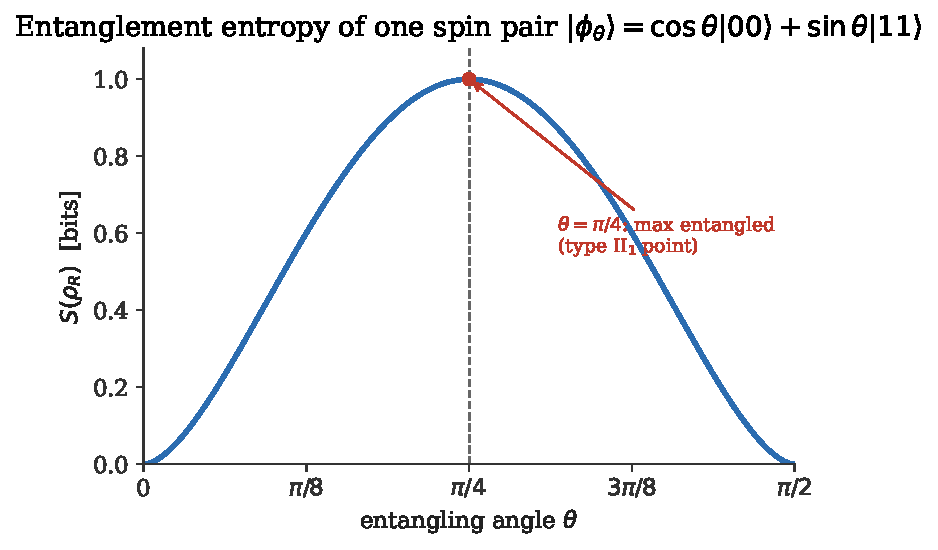
\includegraphics[width=0.75\textwidth]{figs/fig_qubit_entropy.pdf}
\caption{The single-pair entanglement entropy $s_1(\theta) = -\cos^2\theta\log(\cos^2\theta) - \sin^2\theta\log(\sin^2\theta)$ as a function of the mixing angle $\theta \in (0, \pi/4]$. The entropy peaks at the maximally entangled Bell state $\theta = \pi/4$ ($s_1 = \log 2 \approx 0.693$) and vanishes smoothly as $\theta \to 0$. For $N$ pairs, the total entropy scales as $S_R^{(N)} = N s_1(\theta) \to \infty$ as $N \to \infty$.}
\label{fig:qubit_entropy}
\end{figure}

\subsection{The other two examples, more briefly}

The paper gives two more examples (Liu's Ex.~1 and Ex.~3, Sec.~II.A), and it's worth knowing what they are
even in outline, because they come back later — the third one especially, since it's the one that actually
applies to quantum field theory and, ultimately, to AdS/CFT.

\textbf{Ex.~1: lattice gauge theory.} A gauge theory (like electromagnetism, or the strong force) has more
mathematical variables than physical degrees of freedom — you write down a field $U_{ij}$ living on each link
of a lattice, but many different configurations of $U_{ij}$ describe the exact same physics, related by
\emph{gauge transformations} $U_{ij}\to V_iU_{ij}V_j^\dagger$. Physical states are required to be invariant
under these transformations. This requirement — not infinite entanglement, a completely different mechanism —
also breaks the naive tensor factorization $\HH=\HH_R\otimes\HH_L$, because the gauge-invariant states don't,
in general, sit inside a product of an $R$-Hilbert-space and an $L$-Hilbert-space; gauge invariance ties the
two together. This example is flagged explicitly as structurally different from the other two, and it comes
back in Sec.~III.C as a comparatively mild complication (it just adds a classical label — which
gauge/superselection sector you're in — on top of an otherwise ordinary tensor-product story), rather than the
deep, qualitative break that Ex.~2 and Ex.~3 represent.

\textbf{Ex.~3: a quantum field theory cut in half.} Take a relativistic quantum field theory (a scalar field,
say) and split space into two halves, $R=\{x>0\}$ and $L=\{x<0\}$. A quantum field has infinitely many degrees
of freedom packed into any interval of space, however small — informally, a value (or a mode) at every point.
Right at the cutting surface $x=0$, there are infinitely many field degrees of freedom on the $R$ side pressed
arbitrarily close to infinitely many on the $L$ side, all coupled to their immediate neighbors, and this
produces infinite entanglement across the cut in \emph{any} finite-energy state — including the vacuum, the
lowest-energy state there is. This is the field-theory version of exactly the mechanism in Ex.~2 (infinitely
many independent contributions to the entanglement, each one small but adding up to an infinite total), and it
shows up concretely as a divergence: computing the entanglement entropy of the region $R$ with a short-distance
cutoff $\epsilon$ (imagine putting the theory on a lattice with spacing $\epsilon$, which makes everything
finite and well-defined, then asking what happens as $\epsilon\to0$) gives
\[
S_R(\epsilon) = b\,\frac{\mathrm{Area}(\partial R)}{\epsilon^{d-2}} + \cdots, \qquad \epsilon\to0,
\]
(Liu's eq.~2.7) where $\partial R$ is the surface separating $R$ from $L$, $d$ is the spacetime dimension, and
$b$ is some positive, theory-dependent constant. The entropy diverges as the cutoff is removed, and it diverges
in a very specific way — proportional to the \emph{area} of the cutting surface, not its volume. This
``area-law divergence'' is one of the most robust, model-independent facts in quantum field theory (it shows
up in essentially every explicit calculation, from free fields to interacting ones), and this paper's claim is
that it is the direct field-theoretic shadow of exactly the same Hilbert-space-non-factorization phenomenon
as the spin-pair example above — made completely precise later, in Sec.~IV.D, using the language of von
Neumann algebra types.

\begin{figure}[htbp]
\centering
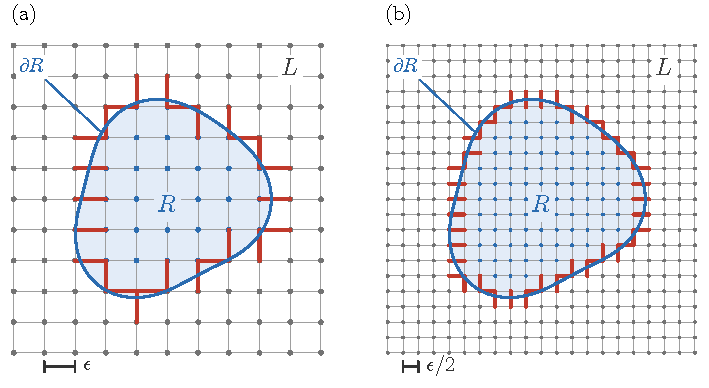
\includegraphics[width=0.75\textwidth]{figs/fig_area_law.pdf}
\caption{The UV area-law divergence of entanglement entropy in quantum field theory: dividing space across a boundary $\partial R$ couples short-distance modes across the cut with UV cutoff $\epsilon$. The leading entanglement entropy diverges as $S_R \sim \mathrm{Area}(\partial R)/\epsilon^{d-2}$, reflecting the infinite entanglement of the underlying Type $\mathrm{III}_1$ local algebra.}
\label{fig:area_law}
\end{figure}

\subsection{Explicit Derivation: Why the Continuum QFT Hilbert Space Cannot Factorize}
\label{sec:qft_nonfactorization_derivation}

Because the claim that ``$\HH \ne \HH_R \otimes \HH_L$ in continuum QFT'' is so fundamental to everything that follows, it is illuminating to derive this result explicitly using nothing more advanced than the quantum mechanics of coupled harmonic oscillators.

\subsubsection*{1. The Hamiltonian and the spatial gradient coupling}

Consider a free, real scalar field $\phi(t, \vec x)$ with mass $m$ in $d$ spacetime dimensions ($d-1$ spatial dimensions). The field Hamiltonian on a constant-time Cauchy slice is
\begin{equation}
H = \int \dd^{d-1}x \left[ \frac{1}{2}\pi(\vec x)^2 + \frac{1}{2}\big(\vec\nabla\phi(\vec x)\big)^2 + \frac{1}{2}m^2\phi(\vec x)^2 \right],
\label{eq:scalar_hamiltonian_continuum}
\end{equation}
where $\pi(\vec x)$ is the canonical momentum field satisfying $[\phi(\vec x), \pi(\vec y)] = i\delta^{(d-1)}(\vec x - \vec y)$.

Now divide space into two halves by a planar boundary at $x = 0$:
\[
R = \{ (x, \vec x_\perp) : x > 0 \}, \qquad L = \{ (x, \vec x_\perp) : x < 0 \},
\]
where $\vec x_\perp = (x^2, \dots, x^{d-1})$ denotes the $(d-2)$ spatial coordinates parallel to the entangling surface $\partial R$.

To isolate the physics right at the boundary, we discretize the perpendicular $x$-direction on a spatial lattice with lattice spacing $\epsilon$, while Fourier-transforming the continuous transverse coordinates $\vec x_\perp$ into transverse momentum modes $\vec k_\perp$:
\[
\phi(x, \vec x_\perp) = \int \frac{\dd^{d-2}k_\perp}{(2\pi)^{d-2}} \, \widetilde\phi(x, \vec k_\perp) \, e^{i \vec k_\perp \cdot \vec x_\perp} .
\]
For each transverse momentum mode $\vec k_\perp$, the Hamiltonian decomposes into an independent 1D chain of coupled harmonic oscillators with effective mass parameter
\begin{equation}
M^2 \equiv m^2 + |\vec k_\perp|^2 .
\label{eq:effective_mass_transverse}
\end{equation}
On the lattice in the $x$-direction, the continuous field becomes discrete site operators $\phi_j(\vec k_\perp) \equiv \widetilde\phi(j\epsilon, \vec k_\perp)$ with conjugate momenta $\pi_j(\vec k_\perp)$, where $j = \dots, -2, -1$ lies in $L$ and $j = 0, 1, 2, \dots$ lies in $R$.

The spatial gradient in the direction perpendicular to the boundary is discretized via finite differences:
\begin{equation}
\int \dd x \, \frac{1}{2}\left(\frac{\partial\phi}{\partial x}\right)^2 \;\longrightarrow\; \sum_j \frac{\epsilon}{2} \left( \frac{\phi_{j+1} - \phi_j}{\epsilon} \right)^2 = \sum_j \frac{1}{2\epsilon} (\phi_{j+1} - \phi_j)^2 .
\label{eq:lattice_gradient_sum}
\end{equation}
Notice the crucial interaction link directly straddling the entangling cut between site $j = -1$ (the closest site in $L$) and site $j = 0$ (the closest site in $R$):
\begin{equation}
H_{\rm cut} = \frac{1}{2\epsilon} (\phi_0 - \phi_{-1})^2 = \frac{1}{2\epsilon} (\phi_R - \phi_L)^2 ,
\label{eq:h_cut_interaction}
\end{equation}
where for clarity we define $\phi_R \equiv \phi_0$ and $\phi_L \equiv \phi_{-1}$.

\subsubsection*{2. The two-oscillator subsystem across the entangling cut}

To see the mechanism with complete clarity, isolate this two-mode system across the interface. The Hamiltonian for these two adjacent oscillators is
\begin{equation}
H_{\rm pair} = \frac{1}{2}\pi_R^2 + \frac{1}{2}\pi_L^2 + \frac{1}{2}M^2(\phi_R^2 + \phi_L^2) + \frac{1}{2\epsilon^2}(\phi_R - \phi_L)^2 .
\label{eq:pair_hamiltonian}
\end{equation}
(Rescaling fields to canonical dimensions $\phi \to \phi/\sqrt{\epsilon}$, $\pi \to \pi\sqrt{\epsilon}$ leaves $[\phi, \pi] = i$ and puts the coupling parameter as $k_{\rm cut} = 1/\epsilon^2$).

Because this is a quadratic system, we diagonalize it exactly using normal mode coordinates:
\begin{equation}
\phi_+ \equiv \frac{\phi_R + \phi_L}{\sqrt{2}}, \qquad \phi_- \equiv \frac{\phi_R - \phi_L}{\sqrt{2}} .
\label{eq:normal_mode_coords}
\end{equation}
In terms of $\phi_\pm$, the Hamiltonian decouples into two uncoupled harmonic oscillators:
\begin{equation}
H_{\rm pair} = \left( \frac{1}{2}\pi_+^2 + \frac{1}{2}\omega_+^2 \phi_+^2 \right) + \left( \frac{1}{2}\pi_-^2 + \frac{1}{2}\omega_-^2 \phi_-^2 \right),
\label{eq:decoupled_pair_hamiltonian}
\end{equation}
whose normal mode eigenfrequencies are
\begin{align}
\omega_+ &= M = \sqrt{m^2 + |\vec k_\perp|^2}, \label{eq:omega_plus} \\
\omega_- &= \sqrt{M^2 + \frac{2}{\epsilon^2}} = \sqrt{m^2 + |\vec k_\perp|^2 + \frac{2}{\epsilon^2}} \approx \frac{\sqrt{2}}{\epsilon} \quad \text{as } \epsilon \to 0 . \label{eq:omega_minus}
\end{align}

\subsubsection*{3. Ground state correlations vs. product state correlations}

The ground state of the decoupled system is the product of two Gaussian ground state wavefunctions in the normal coordinates:
\begin{equation}
\Psi_0(\phi_+, \phi_-) = \left( \frac{\omega_+ \omega_-}{\pi^2} \right)^{1/4} \exp\left[ -\frac{1}{2}\omega_+\phi_+^2 - \frac{1}{2}\omega_-\phi_-^2 \right] .
\label{eq:ground_state_normal}
\end{equation}
Transforming back to the physical local fields $\phi_R, \phi_L$ using eq.~\eqref{eq:normal_mode_coords}:
\begin{align}
\Psi_0(\phi_R, \phi_L) &= \left( \frac{\omega_+ \omega_-}{\pi^2} \right)^{1/4} \exp\left[ -\frac{1}{4}(\omega_+ + \omega_-)(\phi_R^2 + \phi_L^2) - \frac{1}{2}(\omega_+ - \omega_-)\phi_R \phi_L \right] .
\label{eq:ground_state_physical}
\end{align}
Notice the cross-coupling term $\frac{1}{2}(\omega_- - \omega_+)\phi_R \phi_L$. Because $\omega_- \approx \sqrt{2}/\epsilon \gg \omega_+$, this cross-term is extraordinarily large. 

In the true vacuum state $\ket\Omega$:
\begin{itemize}
\item The expectation value of the relative difference between the two sides is suppressed:
\begin{equation}
\braket{\Omega | (\phi_R - \phi_L)^2 | \Omega} = 2 \braket{\Omega | \phi_-^2 | \Omega} = \frac{2}{2\omega_-} = \frac{1}{\omega_-} \approx \frac{\epsilon}{\sqrt{2}} .
\label{eq:vacuum_diff_exp}
\end{equation}
\item The gradient energy of the cut in the vacuum state is therefore finite per mode:
\begin{equation}
\braket{\Omega | H_{\rm cut} | \Omega} = \frac{1}{2\epsilon^2} \braket{\Omega | (\phi_R - \phi_L)^2 | \Omega} = \frac{1}{2\epsilon^2} \frac{1}{\omega_-} \approx \frac{1}{2\sqrt{2}\epsilon} .
\label{eq:vacuum_cut_energy}
\end{equation}
This is the standard zero-point vacuum energy density, which is subtracted when computing excitation energies.
\end{itemize}

\subsubsection*{4. The energetic impossibility of unentangled product states}

Now, suppose for the sake of contradiction that the Hilbert space factorizes across the cut:
\[
\HH \stackrel{?}{=} \HH_L \otimes \HH_R .
\]
If this factorization were valid, the Hilbert space must contain unentangled product states of the form
\begin{equation}
\ket{\Psi_{\rm prod}} = \ket{\psi_L} \otimes \ket{\chi_R} \in \HH ,
\label{eq:hypothetical_product_state}
\end{equation}
where $\ket{\psi_L} \in \HH_L$ and $\ket{\chi_R} \in \HH_R$.

In \emph{any} such product state, by the definition of a tensor product, any operator in $L$ and any operator in $R$ have exactly zero quantum covariance:
\begin{equation}
\braket{\Psi_{\rm prod} | \phi_R \phi_L | \Psi_{\rm prod}} = \braket{\chi_R | \phi_R | \chi_R} \braket{\psi_L | \phi_L | \psi_L} .
\label{eq:product_state_covariance_zero}
\end{equation}
For states with zero mean field ($\braket{\phi_R} = \braket{\phi_L} = 0$, as in any symmetric fluctuation), this means $\braket{\phi_R \phi_L}_{\rm prod} = 0$ identically!

Evaluating the expectation value of the difference squared in this product state gives:
\begin{align}
\braket{\Psi_{\rm prod} | (\phi_R - \phi_L)^2 | \Psi_{\rm prod}} &= \braket{\phi_R^2}_{\chi_R} + \braket{\phi_L^2}_{\psi_L} - 2\braket{\phi_R}_{\chi_R}\braket{\phi_L}_{\psi_L} \nonumber \\
&= \braket{\phi_R^2}_{\chi_R} + \braket{\phi_L^2}_{\psi_L} .
\label{eq:prod_diff_squared}
\end{align}
By the Heisenberg uncertainty principle for each oscillator, the fluctuations are bounded strictly from below:
\[
\braket{\phi_R^2}_{\chi_R} \ge \frac{1}{2\Omega_R}, \qquad \braket{\phi_L^2}_{\psi_L} \ge \frac{1}{2\Omega_L} .
\]
In particular, for any state with localized, finite-energy wavepackets of width $\sim \epsilon$, the single-site fluctuation is bounded by the uncoupled ground state scale:
\begin{equation}
\braket{\Psi_{\rm prod} | (\phi_R - \phi_L)^2 | \Psi_{\rm prod}} \ge \frac{1}{2\omega_+} = \frac{1}{2\sqrt{m^2 + |\vec k_\perp|^2}} = \mathcal{O}(1) \quad (\text{finite, independent of } \epsilon) .
\label{eq:prod_fluctuation_lower_bound}
\end{equation}
Notice the striking difference between eq.~\eqref{eq:vacuum_diff_exp} and eq.~\eqref{eq:prod_fluctuation_lower_bound}:
\begin{itemize}
\item In the entangled vacuum, $\braket{(\phi_R - \phi_L)^2} \sim \mathcal{O}(\epsilon) \to 0$ as the lattice spacing vanishes.
\item In \emph{any} product state, $\braket{(\phi_R - \phi_L)^2} \ge \mathcal{O}(1)$ remains strictly finite as $\epsilon \to 0$, because the absence of entanglement prevents the field values on adjacent sides from fluctuating in lockstep!
\end{itemize}

Now compute the gradient energy across the boundary link in this product state:
\begin{equation}
\braket{\Psi_{\rm prod} | H_{\rm cut} | \Psi_{\rm prod}} = \frac{1}{2\epsilon^2} \braket{\Psi_{\rm prod} | (\phi_R - \phi_L)^2 | \Psi_{\rm prod}} \ge \frac{1}{4\epsilon^2 \sqrt{m^2 + |\vec k_\perp|^2}} .
\label{eq:hcut_prod_divergence}
\end{equation}
Subtracting the vacuum zero-point energy (eq.~\eqref{eq:vacuum_cut_energy}), the excess excitation energy required to sever the entanglement of this single transverse mode across the cut is
\begin{equation}
\Delta E_{\rm cut}(\vec k_\perp) = \braket{\Psi_{\rm prod} | H_{\rm cut} | \Psi_{\rm prod}} - \braket{\Omega | H_{\rm cut} | \Omega} \ge \frac{1}{4M\epsilon^2} - \frac{1}{2\sqrt{2}\epsilon} \sim \frac{1}{4M\epsilon^2} > 0 .
\label{eq:delta_e_single_mode}
\end{equation}

\subsubsection*{5. Integration over the entangling surface and the non-factorization theorem}

To obtain the total excitation energy required to prepare the unentangled product state $\ket{\psi_L}\otimes\ket{\chi_R}$ across the entire boundary surface $\partial R$, we integrate $\Delta E_{\rm cut}(\vec k_\perp)$ over all transverse spatial coordinates $\vec x_\perp$, or equivalently over all transverse momentum modes $|\vec k_\perp| \le \Lambda_{\rm UV} \sim 1/\epsilon$:
\begin{align}
\Delta E_{\rm prod} &= \mathrm{Area}(\partial R) \int_{|\vec k_\perp| \le 1/\epsilon} \frac{\dd^{d-2}k_\perp}{(2\pi)^{d-2}} \, \Delta E_{\rm cut}(\vec k_\perp) \nonumber \\
&\ge \mathrm{Area}(\partial R) \int_{|\vec k_\perp| \le 1/\epsilon} \frac{\dd^{d-2}k_\perp}{(2\pi)^{d-2}} \, \frac{1}{4\epsilon^2 \sqrt{m^2 + |\vec k_\perp|^2}} .
\label{eq:total_prod_energy_integral}
\end{align}
Evaluating the radial momentum integral in $d$ spacetime dimensions ($d \ge 3$):
\[
\int_0^{1/\epsilon} k_\perp^{d-3} \frac{\dd k_\perp}{k_\perp} \sim \int_0^{1/\epsilon} k_\perp^{d-4} \dd k_\perp \sim \left(\frac{1}{\epsilon}\right)^{d-3} .
\]
Multiplying by the prefactor $\frac{1}{\epsilon^2}$:
\begin{keyresult}
\begin{equation}
\Delta E_{\rm prod} \ge C \cdot \frac{\mathrm{Area}(\partial R)}{\epsilon^{d-1}} \;\xrightarrow{\;\epsilon \to 0\;} \; +\infty ,
\label{eq:product_state_energy_divergence}
\end{equation}
where $C > 0$ is a strictly positive, theory-dependent geometric constant.
\end{keyresult}

Equation~\eqref{eq:product_state_energy_divergence} is the definitive physical proof of non-factorizability:
\begin{enumerate}
\item \textbf{Infinite energy barrier}: The physical energy required to unentangle a spatial subregion $R$ from its complement $L$ diverges as $\epsilon^{-(d-1)}$ in the continuum limit. Any attempt to enforce a tensor product state requires creating an infinite gradient discontinuity at $\partial R$.
\item \textbf{Expulsion from the physical Hilbert space}: The physical Hilbert space $\HH$ of a continuum quantum field theory consists solely of finite-energy states (mathematically, states in the Fock space or GNS space of the vacuum). Because $\Delta E_{\rm prod} = +\infty$, \emph{no product states exist anywhere within $\HH$}.
\item \textbf{Failure of factorization}: A tensor product $\HH_L \otimes \HH_R$ is, by definition, spanned by product vectors $\ket{\psi_L}\ket{\chi_R}$. Because $\HH$ contains zero product vectors, we reach an inescapable mathematical conclusion:
\begin{equation}
\boxed{\HH \ne \HH_L \otimes \HH_R \quad \text{in any continuum relativistic quantum field theory.}}
\label{eq:non_factorization_conclusion}
\end{equation}
\end{enumerate}

\subsubsection*{6. The algebraic corollary: Type $\mathrm{III}_1$ and the split property}

This energetic divergence explains why local subregions in QFT cannot be described by Type I algebras:
\begin{itemize}
\item If two spatial regions $R_1$ and $R_2$ are separated by a \textbf{finite buffer distance} $\delta > 0$ (so $\text{dist}(R_1, R_2) = \delta$), the gradient energy across the gap is regularized by $\delta$. In that case, an unentangled product state \emph{can} be prepared, but at an energy cost scaling as $\exp(c/\delta^n)$. The mathematical statement that product states exist for strictly separated regions is known in axiomatic QFT as the \textbf{Doplicher--Longo split property}: there exists an intermediate Type I factor $\mathcal{N}$ such that $\M(R_1) \subset \mathcal{N} \subset \M(R_2')'$.
\item However, as the buffer distance is sent to zero ($\delta \to 0$, so the regions touch at a common boundary), the split property collapses, the energy diverges to $+\infty$, and the local algebra $\M(R)$ ceases to be Type I or Type II — it becomes an intrinsically entangled \textbf{Type $\mathrm{III}_1$ factor}.
\end{itemize}

\subsection{The fix: define a subsystem by what you can \emph{do}, not by how you'd \emph{split the Hilbert
space}}

Here is the resolution the paper proposes, and it is worth sitting with how simple the idea actually is
before any formalism gets attached to it. Instead of defining a subsystem $R$ by declaring a factorization
$\HH=\HH_R\otimes\HH_L$ up front, define it operationally: \emph{$R$ is whatever an observer confined to
that subsystem can measure or do.} Concretely, that observer has access to some collection of operators
$\M\subset B(\HH)$ (the set of all bounded operators on the full Hilbert space $\HH$) — every self-adjoint
combination of things their apparatus can measure, and every unitary transformation their apparatus can
apply. Nothing about this definition requires $\HH$ to factor into anything. It only requires that you can
say, of any given operator, whether or not it belongs to the observer's toolkit.

This reframing costs nothing in the ordinary case (when $\HH=\HH_R\otimes\HH_L$ genuinely does exist, the
natural choice $\M=B(\HH_R)\otimes\id_L$ — every operator acting only on $R$ — recovers exactly the familiar
picture, as you'll see made precise in the next section), and it costs nothing in the broken case either,
because ``the set of operators an $R$-observer can apply'' is a perfectly sensible, well-defined thing to talk
about even when there's no factorization for it to come from. You lose nothing and gain a definition that
survives exactly the cases where the old one dies.

Naming what kind of mathematical object $\M$ should be — closed under sums, products, and the operation of
taking a Hermitian conjugate, plus some notion of being closed under limits — is precisely what a
\textbf{von Neumann algebra} is, and pinning down exactly which notion of ``limit'' is the right one (there
turn out to be two inequivalent choices, and the difference matters enormously) is the entire content of the
next section, Sec.~II.

This is, historically, not a new invention grafted onto quantum mechanics from outside. In the late 1920s and
early 1930s, John von Neumann — one of the people who built the mathematical foundations of quantum mechanics
in the first place, the same person behind the ``Dirac--von Neumann axioms'' you may have seen stated in
Sakurai — worked out, together with Francis Murray, a complete classification of exactly these kinds of
operator algebras. For decades this classification lived mostly inside pure mathematics. The claim of this
paper (built on work going back to Rehren in the 1990s, and developed intensively since roughly 2021 by
Leutheusser, Liu, and others) is that this same 1930s classification, when applied to the algebra $\M$ of an
observer's accessible operators, is \emph{exactly} a classification of how entangled that observer's
subsystem is with everything they cannot access — turning an abstract piece of 1930s functional analysis into
a working tool for 2020s quantum gravity.

\subsection{Two organizing claims, and how seriously to take them at this stage}

The paper states its two central claims very early (its eq.~1.3 and the paragraph after it), and it is useful
to know, right at this stage, exactly how much has been established when you first read them, versus how much
is being promised for later. Restated:

\begin{center}
\emph{Classifying von Neumann algebras} $\;\longleftrightarrow\;$ \emph{classifying broad types of
entanglement.}
\end{center}

and, going beyond this broad classification, finer tools from the same theory (modular theory, covered in
Sec.~IV, and the crossed product, covered in Sec.~V) are claimed to give access to much sharper entanglement
information than the broad type alone.

At the point in the paper where these claims first appear, they are \emph{stated}, not yet demonstrated. Don't
mistake the double-headed arrow above for a formal theorem with a name and a citation — it isn't one. It's a
dictionary that gets built up, entry by entry, over Secs.~III and IV: each von Neumann algebra type (I, then
II, then the various subtypes of III) is matched, on specific worked examples, to a specific qualitative
pattern of entanglement between a subsystem and its complement. By the time you finish Sec.~IV you will have
seen this correspondence demonstrated concretely enough, on examples you can check by hand, that the arrow in
eq.~1.3 will feel earned rather than asserted. That is exactly the arc this companion follows too — the
promise made here in Sec.~I is redeemed piece by piece, not all at once.

Similarly, the deeper claim that entanglement structure is what \emph{builds} bulk spacetime geometry — the
subregion-subalgebra duality that gives this paper its title — is motivated here by pointing at the
Ryu--Takayanagi formula and the broader ``entanglement builds geometry'' literature (Van~Raamsdonk
\cite{VanRaamsdonk}, Maldacena--Susskind \cite{MaldacenaSusskind}), but the actual mechanism — \emph{why} a
boundary algebra of a specific type turns out to be identical, not just related, to a bulk causal region's
algebra of observables — isn't built until Sec.~VII. Reading Sec.~I as ``a map of where we're going and why
people believe it's worth going there,'' rather than as a self-contained argument, is the right way to read
it; that's genuinely all a paper's introduction can do.

\subsection{Sec.~I.A: the plan of the article, translated}

The paper's own plan (p.~6) splits its ten sections into two halves. It's worth restating in a way that says
\emph{why} the split falls where it does, since the reason is itself informative about how the argument is
built.

\textbf{Secs.~II--V: the mathematics, with no gravity or holography anywhere in sight.} This half is pure
operator-algebra theory, developed using only ordinary, finite-dimensional-friendly quantum mechanics
examples (mostly the entangled-spin-pair system from above). Sec.~II lays down what a von Neumann algebra is
and how they're classified. Secs.~III and IV show, type by type, how that classification tracks entanglement
structure — Sec.~III handles the ``easy'' types (I and II, where a density matrix and an entropy can still be
defined), and Sec.~IV handles type III, which cannot be tamed by a density matrix at all and needs an entirely
new tool (Tomita--Takesaki modular theory) to say anything quantitative about it. Sec.~V introduces the
\emph{crossed product}, a construction that takes a type III algebra and, by literally attaching an auxiliary
quantum clock to it, produces a new, better-behaved type II algebra out of it — a purely algebraic trick at
this stage, with no physical motivation given yet, but one that turns out (starting in Sec.~IX) to be exactly
what a real physical observer, carrying a real physical clock, is doing to gravitational observables.

\textbf{Secs.~VI--IX: applying all of that machinery to quantum gravity.} Sec.~VI sets up the large-$N$
algebraic formulation of AdS/CFT itself. Sec.~VII introduces subregion-subalgebra duality — the paper's
central physics claim, that a bulk spacetime region and a specific boundary operator algebra are literally the
same object, described in two languages — and uses it to reformulate entanglement-wedge and causal-wedge
reconstruction (ideas you may already have encountered in AdS/CFT courses) in this new algebraic language.
Sec.~VIII shows how bulk causal structure, horizons, and even the question of whether two disconnected
boundary theories are joined by a wormhole, can all be read directly off the type and commutant structure of
boundary algebras, with no bulk metric assumed anywhere. Sec.~IX builds simple, fully solvable toy models
(observers with real physical clocks, crossed by the modular group exactly as in Sec.~V) that reproduce black
hole and de~Sitter entropy from nothing but this operator-algebraic machinery.

\subsection{Sec.~I.B: conventions and notation, explained rather than just listed}

This short subsection (p.~8 of the paper) is easy to skim past, but every single item in it gets used, without
further comment, dozens of times later — so it's worth actually understanding each one now rather than
looking it up under pressure in Sec.~VII.

\begin{itemize}
\item \textbf{Large $N$ vs.\ finite $N$.} ``Large-$N$'' (equivalently $G_N\to0$) means doing a perturbative
expansion in powers of $1/N$ — you can keep more than just the very first (leading) term, but you're still
fundamentally treating $1/N$ as a small parameter you expand in, the same way you'd do ordinary perturbation
theory in quantum mechanics. ``Finite $N$'' (finite $G_N$) means the opposite: treating $N$ (or $G_N$) as an
honest, fixed number, with no expansion at all — the genuinely nonperturbative, full quantum-gravity regime.
Most of this paper works at large $N$; finite-$N$ questions are the hardest open problems, touched on mainly
in Secs.~VII.F and IX.D.

\item \textbf{$\HH$, $B(\HH)$, and boundedness.} $\HH$ is a Hilbert space (a complex vector space with an
inner product, complete under the norm that inner product defines — the same notion you already know from
ordinary quantum mechanics, just possibly infinite-dimensional). $B(\HH)$ is the set of \emph{bounded}
operators on $\HH$: an operator $A$ is bounded if there's some finite number $c$ such that $\|A\ket\psi\|\le
c\|\ket\psi\|$ for every vector $\ket\psi\in\HH$ — informally, $A$ never stretches a vector's length by more
than a fixed factor, no matter which vector you feed it. Ordinary finite matrices are automatically bounded.
Some familiar quantum-mechanical operators are \emph{not} bounded — position $\hat x$ and momentum $\hat p$ on
a particle on a line, for instance, can make $\|A\ket\psi\|/\|\ket\psi\|$ as large as you like by choosing
$\ket\psi$ spread out far enough, or oscillating fast enough. The paper sidesteps this by simply restricting
attention to bounded operators throughout, and noting that in field theory any operator you actually care
about can be suitably smeared/regularized to become bounded (e.g., $e^{i\hat x}$ is bounded even though
$\hat x$ itself is not). This restriction is not a loss of generality worth worrying about; it's a standard
technical convenience that lets the norm-based definitions below (Sec.~II.B.1) work cleanly.

\item \textbf{$\id$} is the identity operator — ``do nothing.''

\item \textbf{$\widetilde J^\pm(Y)$: causal future and past.} For a region $Y$ in a spacetime, $\widetilde
J^+(Y)$ is the set of every point that can be reached from some point of $Y$ by a future-directed causal
curve — a path that never moves faster than light and always moves forward in time. Physically: everything $Y$
could possibly send a signal to, given unlimited time. $\widetilde J^-(Y)$ is the mirror image: everything
that could have sent a signal to some point of $Y$. (The tilde signals that these are computed in the
\emph{conformal completion} of the spacetime — a technical device, standard in the AdS/CFT literature, that
adds a boundary ``at infinity'' so that causal curves reaching arbitrarily far away are still tracked
properly; you can safely picture ordinary causal future/past for now and revisit the tilde once conformal
compactification actually matters, starting around Sec.~VI.)

\item \textbf{Causal complement (single prime) and causal completion (double prime), on a spacetime region.}
The causal complement $Y'$ of a region $Y$ is everything that is spacelike separated from all of $Y$ — every
point that cannot send or receive a signal to or from any point of $Y$ within the time available; loosely,
``everything $Y$ has absolutely no causal influence on, in either direction.'' The causal completion $Y''$ is
the double complement, $(Y')'$ — and (this is a genuinely important geometric fact, not just a notational
curiosity) $Y''$ is generally \emph{larger} than $Y$ itself: it's the largest region that has exactly the same
causal future and past as $Y$ does. A single point on a Cauchy slice, for instance, has a causal completion
equal to the single point itself (nothing to add), but a spatial region $R$ on a Cauchy slice has a causal
completion equal to its entire \emph{domain of dependence} (defined next) — a genuinely bigger set, extending
into the past and future. This double-prime notation for spacetime regions is deliberately built to echo the
double-prime notation for operator commutants ($\M''$) that you'll meet in the very next section, and the
paper is relying on that echo: causal completion of a region and double-commutant closure of an algebra turn
out, once subregion-subalgebra duality is established in Sec.~VII, to be two faces of the same fact.

\item \textbf{$\bar R$, complement of a spatial region; $\hat R$, domain of dependence.} If $R$ is a subregion
of a single spatial slice (a snapshot of space at one moment), $\bar R$ is just its ordinary set-complement on
that slice — everything on the same slice that isn't in $R$. $\hat R$, the domain of dependence, is a genuinely
spacetime notion built from $R$: it's every spacetime point $p$ such that \emph{every} causal curve through
$p$ — no matter which direction it goes, as long as it never exceeds the speed of light — must cross $R$. This
is exactly the region whose entire future \emph{and} past history is completely determined by data specified
on $R$ alone, which is why it's called the domain of \emph{dependence}: physics inside $\hat R$ depends only on
initial data given on $R$. For $R$ a full spatial slice, $\hat R$ is the entire spacetime. For $R$ a proper
subregion, $\hat R$ is a diamond-shaped region (a \emph{causal diamond}) sitting above and below $R$, bounded
by the light rays that just barely graze the edge of $R$. This shape shows up constantly from Sec.~VI onward;
it's worth actually picturing it once here.

\item \textbf{$\subset$ always means \emph{proper} subset.} A small notational point that matters: whenever
you see $\M_1\subset\M_2$ in this paper, it means $\M_1$ is strictly smaller than $\M_2$ (not equal to it) —
not the more permissive convention (allowing equality) some other texts use for the same symbol.
\end{itemize}

With this vocabulary in hand — bounded operators, causal future/past, causal complement and completion,
domain of dependence — you have everything you need to read the rest of the paper's geometric statements
literally, rather than by pattern-matching to what looks familiar. The next section builds the algebraic
machinery ($C^*$ and von Neumann algebras, states, projections, the type classification, and the GNS
construction that produces a Hilbert space from an algebra) that this section's discussion has been building
toward.
